\documentclass[a4paper]{article}
\usepackage[utf8]{vietnam}
\usepackage[left=3cm,right=2cm,top=2cm,bottom=2cm]{geometry}
\usepackage{amsmath}
\setlength{\parindent}{0pt}
\usepackage{graphicx} 
\usepackage{multirow}
\usepackage{url}
%\usepackage{wallpaper}
%\usepackage[firstpage]{draftwatermark} 
\usepackage{xcolor}
\usepackage{tikz} 
\usepackage{scrextend}
\usepackage{ulem}
\changefontsizes{13pt}
%\usepackage{background}
\usetikzlibrary{calc}
\usepackage{fancyhdr}
% \usepackage[sorting=none]{biblatex}
% \addbibresource{references.bib}

\usepackage{titlesec}
\usepackage{enumitem}
\usepackage{amsmath}
\titleformat{\section}{\fontsize{13}{15}\selectfont\bfseries}{\thesection}{1em}{}
\titleformat{\subsection}{\fontsize{13}{15}\selectfont\bfseries}{\thesubsection}{1em}{}

%----------------------- config của sy-------------
\usepackage{setspace}
\onehalfspacing
\usepackage{float}
\restylefloat{figure}
\floatplacement{figure}{H}
\usepackage{indentfirst}
\setlength{\parindent}{1cm}
%--------------------------------------Header footer------------------------------------
\pagestyle{fancy}
\fancyhf{} % Xóa định dạng hiện tại của header và footer

% Header
\lhead{Ứng dụng Machine Learning để phân loại lá cây}
\chead{}
\rhead{GVHD: Hoàng Lê Uyên Thục}

% Footer
\lfoot{Báo cáo cuối kỳ: Trí tuệ nhân tạo}
\cfoot{} % Hiển thị số trang ở giữa footer
\rfoot{Trang \thepage}

% Định dạng các đường line ở header và footer
\renewcommand{\headrulewidth}{0.1pt} % Độ dày của đường line ở header
\renewcommand{\footrulewidth}{0.1pt} % Độ dày của đường line ở footer
%---------------------------------------------------------------------------------------
%\backgroundsetup{scale = 1, angle = 0, opacity = 0.2,
%contents = {\includegraphics[width = 0.9\paperwidth,
%height = 0.9\paperheight, keepaspectratio] {hust.png}}}

%\backgroundsetup{scale = 1, angle = 0, opacity = 0.2,
%contents = {\includegraphics[width = 0.97\paperwidth,
%height = 0.97\paperheight, keepaspectratio] {bia.png}}}
\begin{document}

\begin{titlepage}
%\SetWatermarkText{\includegraphics[width = 0.97\paperwidth,
%height = 0.97\paperheight]{bia.png}}
%\SetWatermarkAngle{0} 
%\SetWatermarkText{\includegraphics[scale=1]{hust.png}}
%\SetWatermarkAngle{0} 
\begin{tikzpicture}[remember picture,overlay,inner sep=0,outer sep=0]
     \draw[black!80!black,line width=4pt] ([xshift=-2cm,yshift=-2cm]current page.north east) coordinate (A)--([xshift=3cm,yshift=-2cm]current page.north west) coordinate(B)--([xshift=3cm,yshift=2cm]current page.south west) coordinate (C)--([xshift=-2cm,yshift=2cm]current page.south east) coordinate(D)--cycle;

     \draw ([yshift=0.5cm,xshift=-0.5cm]A)-- ([yshift=0.5cm,xshift=0.5cm]B)--
     ([yshift=-0.5cm,xshift=0.5cm]B) --([yshift=-0.5cm,xshift=-0.5cm]B)--([yshift=0.5cm,xshift=-0.5cm]C)--([yshift=0.5cm,xshift=0.5cm]C)--([yshift=-0.5cm,xshift=0.5cm]C)-- ([yshift=-0.5cm,xshift=-0.5cm]D)--([yshift=0.5cm,xshift=-0.5cm]D)--([yshift=0.5cm,xshift=0.5cm]D)--([yshift=-0.5cm,xshift=0.5cm]A)--([yshift=-0.5cm,xshift=-0.5cm]A)--([yshift=0.5cm,xshift=-0.5cm]A);

     \draw ([yshift=-0.3cm,xshift=0.3cm]A)-- ([yshift=-0.3cm,xshift=-0.3cm]B)--
     ([yshift=0.3cm,xshift=-0.3cm]B) --([yshift=0.3cm,xshift=0.3cm]B)--([yshift=-0.3cm,xshift=0.3cm]C)--([yshift=-0.3cm,xshift=-0.3cm]C)--([yshift=0.3cm,xshift=-0.3cm]C)-- ([yshift=0.3cm,xshift=0.3cm]D)--([yshift=-0.3cm,xshift=0.3cm]D)--([yshift=-0.3cm,xshift=-0.3cm]D)--([yshift=0.3cm,xshift=-0.3cm]A)--([yshift=0.3cm,xshift=0.3cm]A)--([yshift=-0.3cm,xshift=0.3cm]A);

   \end{tikzpicture}


\begin{center}
    \vspace{7pt}
    \fontsize{14pt}{16pt}
    \textbf{TRƯỜNG ĐẠI HỌC BÁCH KHOA - ĐẠI HỌC ĐÀ NẴNG}
    
    \vspace{7pt}
    \textbf{KHOA ĐIỆN TỬ - VIỄN THÔNG}
\end{center}
\vspace{10pt}
\begin{center}
    \includegraphics[scale=0.37]{images/logodut.jpg}
    \includegraphics[scale=0.75]{images/logoete.jpg}
    
    \vspace{20pt}
    \fontsize{20pt}{17pt}\selectfont 
    \textbf{BÁO CÁO CUỐI KỲ} \\
    \vspace{7pt}
    \textbf{Học phần: Trí tuệ nhân tạo}
    \vspace{7pt}
    % \textbf{PBL3: MẠNG MÁY TÍNH}
\end{center}
\begin{flushleft}
    \fontsize{15pt}{10pt}\selectfont  
    \textbf{\textsl{\hspace{27pt}{\uline{ĐỀ TÀI:}}}}
\end{flushleft} 
\begin{center}
    \fontsize{16pt}{17pt}\selectfont 
    \textbf{\textrm{Ứng dụng Machine Learning để phân loại lá cây}}
\end{center}

\vspace{50pt}
\begin{addmargin}[1cm]{0cm}
\textbf{Giảng viên hướng dẫn: \hspace{2cm}Hoàng Lê Uyên Thục}
\end{addmargin}
\vspace{10pt}
% Bảng sinh viên thực hiện thụt vào 2cm
\begin{addmargin}[1cm]{0cm}
\textbf{Sinh viên thực hiện: \hspace{2.6cm}NHÓM 2}
\begin{tabbing}
\hspace{4cm}\=\hspace{3cm}\=\hspace{5cm} \kill
{\textbf{Họ và tên}}\>{\textbf{MSSV}}\>{\textbf{Email liên hệ}}\\
\hspace{4cm}\=\hspace{3cm}\=\hspace{5cm} \kill
Lê Phạm Công\> 106200221\> 106200221@sv1.dut.udn.vn\\
\hspace{4cm}\=\hspace{3cm}\=\hspace{5cm} \kill
Phan Công Danh\> 106200222\> 106200222@sv1.dut.udn.vn\\
\hspace{4cm}\=\hspace{3cm}\=\hspace{5cm} \kill
Đoàn Thế Lên\> 106200233\> 106200233@sv1.dut.udn.vn\\
\hspace{4cm}\=\hspace{3cm}\=\hspace{5cm} \kill
Lê Minh Nhật\> 106200238\> 106200238@sv1.dut.udn.vn\\
\end{tabbing}
\end{addmargin}
\vspace{2.5cm}
\begin{center}
    \textbf{Đà Nẵng, ngày 31 tháng 05 năm 2023}
\end{center}
\end{titlepage}
% -------------------------------------End trang bìa-----------------------
\newpage
\tableofcontents
\newpage

% ----------------------- MAIN DOCUMENT---------------------------%
\section*{Tóm tắt}
\addcontentsline{toc}{section}{Tóm tắt}
Nghiên cứu này nhằm phân loại ba loại lá cây \textit{Cercis chinensis}, \textit{Indigofera tinctoria}, và \textit{Acer palmatum} nằm trong bộ dữ liệu Flavia được công bố tại \cite{wu2007leaf} bằng cách sử dụng hai kỹ thuật học máy, K-Nearest Neighbors (KNN) và Support Vector Machine (SVM), với hai loại đặc trưng khác nhau: Moment Invariants (HU's Moments) và Histogram of Oriented Gradients (HOG). Đặc trưng HU's Moments được sử dụng để nắm bắt các đặc trưng hình học cơ bản của lá cây, đảm bảo tính bất biến với phép quay, dịch chuyển và tỷ lệ, trong khi đặc trưng HOG được áp dụng để trích xuất các thông tin về hình dạng và cấu trúc thông qua phân bố của các gradient hướng trong hình ảnh. 

Các kết quả thu được khi lần lượt sử dụng KNN và SVM trên từng loại đặc trưng HOG và HU's Moments rất khả quan. Với HOG, KNN cho kết quả accuracy là 94.64\%, SVM là 100\%. Với HU's Moments, KNN mang lại accuracy  là 100\%, SVM là 99.5\%. Đồng thời các chỉ số khác là Precision, Recall, F1-Score đều rất cao mặc dù có sự chênh lệch nhỏ với từng mô hình và loại đặc trưng.

Mã nguồn của báo cáo có thể được tìm thấy tại \url{https://github.com/lephamcong/Classification_Of_Leaves.git}


\section{Giới thiệu}
Phân loại các loài thực vật dựa trên hình ảnh lá cây là một lĩnh vực nghiên cứu quan trọng trong khoa học máy tính và sinh học thực vật, với ứng dụng rộng rãi trong nhiều lĩnh vực như nông nghiệp, bảo tồn sinh học, và nghiên cứu môi trường. Sự phát triển của các kỹ thuật học máy đã mở ra nhiều cơ hội mới cho việc phân loại và nhận dạng thực vật một cách tự động và chính xác.

Một trong những phương pháp phổ biến để trích xuất đặc trưng từ hình ảnh lá cây là sử dụng Moment Invariants (HU's Moments). Các đặc trưng HU's Moments, được giới thiệu vào năm 1962 trong tài liệu \cite{hu1962}, là một bộ các đặc trưng hình học bất biến với các phép biến đổi hình học như quay, dịch chuyển và tỷ lệ. 

Một phương pháp khác để trích xuất đặc trưng là Histogram of Oriented Gradients (HOG), được phát triển và công bố trong tài liệu \cite{hog2005}. Đặc trưng HOG tập trung vào việc phân tích sự phân bố của các gradient hướng trong hình ảnh, giúp nắm bắt các chi tiết hình dạng và cấu trúc phức tạp. 

Các kỹ thuật học máy như K-Nearest Neighbors (KNN) và Support Vector Machine (SVM) đã được sử dụng rộng rãi trong phân loại hình ảnh. KNN là một phương pháp phân loại không tham số dựa trên khoảng cách giữa các điểm dữ liệu, trong khi SVM sử dụng các siêu phẳng để phân chia không gian đặc trưng và phân loại dữ liệu.

Các tác giả của \cite{svm-and-knn} đã so sánh hiệu quả của KNN và SVM trong việc phân loại lá nho khỏe mạnh và không khỏe mạnh và phát hiện ra rằng đối với ảnh thời gian thực, KNN (với K=1) cho độ chính xác cao hơn so với SVM. Độ chính xác của hệ thống đề xuất trong \cite{svm-and-knn} đạt được là 90\% đối với bộ phân loại SVM và 96,66\% đối với bộ phân loại KNN.Điều đó đã chứng tỏ sự hiệu quả của KNN và SVM trong giải quyết các bài toán phân loại. 

Nghiên cứu này nhằm đánh giá hiệu quả của các kỹ thuật KNN và SVM trong việc phân loại ba loại lá cây: Cercis chinensis, Indigofera tinctoria, và Acer palmatum, sử dụng hai loại đặc trưng khác nhau: HU's Moments và HOG. Mục tiêu của nghiên cứu là so sánh hiệu suất của các phương pháp phân loại và xác định phương pháp tối ưu cho từng loại đặc trưng. Kết quả của nghiên cứu này không chỉ góp phần nâng cao hiểu biết về khả năng phân loại lá cây mà còn mở ra hướng đi mới cho việc ứng dụng học máy trong phân loại thực vật.

\section{Phương pháp}
\begin{figure}
    \centering
    \includegraphics[width=1\linewidth]{images/sodohethong.png}
    \caption{Sơ đồ tổng quan}
    \label{fig:sodohethong}
\end{figure}

Hình \ref{fig:sodohethong} thể hiện tổng quan về phương pháp thực hiện trong nghiên cứu này. Dữ liệu được sử dụng là dữ liệu về 3 loại lá cây Cercis chinensis với 72 mẫu, Indigofera tinctoria với 73 mẫu và Acer palmatum với 56 mẫu được lấy từ bộ dữ liệu Flavia \cite{wu2007leaf}. Dữ liệu được chuẩn bị là dữ liệu ảnh có kích thước 1600x1200 pixels, dữ liệu cần được tiến hành các bước tiền xử lý theo yêu cầu của quá trình trích xuất đặc trưng HOG và HU's Moment. Dữ liệu được trích xuất đặc trưng theo từng loại và gán nhãn theo quy ước: Cercis chinensis sẽ gắn nhãn là 4, Indigofera tinctoria gắn nhãn là 5 và Acer Palmatum sẽ gắn nhãn là 6, đây là quy ước riêng trong nghiên cứu này, nhãn này có thể tùy chọn theo yêu cầu của từng bài toán khác nhau. Các đặc trưng sau khi được trích xuất và gắn nhãn sẽ sử dụng làm dữ liệu cho các mô hình phân loại như Hình \ref{fig:sodohethong}. Kết quả sẽ được tổng hợp và đánh giá theo từng mô hình phân loại và theo từng đặc trưng.

\subsection{Đặc trưng HOG (Histogram of Oriented Gradients)} 
Histogram of Oriented Gradients (HOG) được đề cập trong \cite{hog2005} là là một kỹ thuật phổ biến trong lĩnh vực thị giác máy tính và xử lý ảnh, được sử dụng để mô tả và phát hiện các đặc trưng quan trọng của các vật thể trong hình ảnh.

HOG dựa trên việc nhận dạng hình dạng của đối tượng cục bộ qua việc sử dụng hai ma trận quan trọng: ma trận độ lớn của gradient và ma trận hướng của gradient.  
\begin{figure}
    \centering
    \includegraphics[width=1\linewidth]{images/sodohog.png}
    \caption{Sơ đồ quá trình trích xuất đặc trưng HOG}
    \label{fig:sodohog}
\end{figure}

Hình \ref{fig:sodohog} mô tả quá trình trích xuất đặc trưng HOG, chi tiết quá trình trích xuất đặc trưng như sau:
\begin{itemize}[label={}]
    \item \textbf{Bước 1: }Ảnh đầu vào được chuyển sang dạng ảnh xám nhị phân và resize kích thước về 160x120pixels để giảm kích thước dữ liệu giúp đơn giản hóa quá trình xử lý và tập trung vào cấu trúc hình dạng của vật thể mà không bị ảnh hưởng bởi màu sắc. Việc thay đổi kích thước ảnh về 1 kích thước giúp thống nhất các đầu vào trong trường hợp dữ liệu chưa thống nhất. 
    \item \textbf{Bước 2: }Tính gradient của ảnh được thực hiện bằng cách sử dụng các mặt nạ lọc, mặt nạ 3x3 được sử dụng phổ biến. Mặt nạ lọc thông dụng là mặt nạ Sobel 3x3 tính gradient theo hai hướng (x và y), và sau đó sử dụng các gradient này để tính toán các đặc trưng HOG. 
    \item \textbf{Bước 3: }Biểu diễn đặc trưng của ảnh thông qua 2 thông số liên quan đến mức độ thay đổi cường độ màu sắc (gradient magnitude) và hướng thay đổi cường độ màu sắc (gradient direction).
    \item \textbf{Bước 4: }Tạo một bộ mô tả có thể chuyển ảnh thành vector thể hiện thông tin của gradient magnitude và gradient direction. Một biểu đồ Histogram thống kê độ lớn Gradient sẽ được tính toán trên mỗi ô cục bộ. Kích thước mỗi ô là 8x8pixels, Histogram của gradient có 9 thanh, mỗi khối là 2x2 ô và phần chồng lấn giữa các khối là 1x1 ô. 
    \item \textbf{Bước 5: }Chuẩn hóa Histogram của Gradient bằng chuẩn L2-Hys (sự kết hợp giữa chuẩn L2 và kỹ thuật hysteresis để đảm bảo rằng các vector đặc trưng được chuẩn hóa tốt và tránh được các vấn đề liên quan đến giá trị gradient quá nhỏ hoặc quá lớn).
    \item \textbf{Bước 6: }Xuất ra vector đặc trưng của ảnh. Trong phạm vi nghiên cứu này, ảnh đầu vào được resize thành 160x120 pixels, kích thước 1 ô là 8x8 pixels, kích thước khối là 2x2 ô, 9 giá trị/ 1 ô. Suy ra Vector đặc trưng có số chiều là [1, 9576].
\end{itemize}
Hình \ref{fig:hogfeature} thể hiện vector đặc trưng HOG của 1 mẫu dữ liệu trong mỗi loại lá cây. 
\begin{figure}
    \centering
    \includegraphics[width=0.75\linewidth]{images/hogfeature.png}
    \caption{vector đặc trưng HOG của 3 loại lá cây}
    \label{fig:hogfeature}
\end{figure}
\newpage
\subsection{Đặc trưng HU's Moments}
Hu’s moments (Hu’s moment invariants) là một tập hợp gồm 7 số được tính bằng cách sử dụng khoảnh khắc trung tâm (central moments) bất biến đối với các phép biến đổi hình ảnh. 6 khoảnh khắc đầu tiên đã được chứng minh là bất biến đối với chuyển động tịnh tiến, tỷ lệ, xoay và phép lật. Trong khi dấu hiệu của khoảnh khắc thứ 7 thay đổi để phản ánh hình ảnh.
\begin{figure}
    \centering
    \includegraphics[width=1\linewidth]{images/sodohu.png}
    \caption{Sơ đồ quá trình trích xuất đặc trưng HU's Moments}
    \label{fig:sodohu}
\end{figure}
Để tính được HU's Moment ảnh cần được chuẩn hóa về cùng một kích thước ảnh (nghiên cứu này sử dụng kích thước 1600x1200 pixels để tính HU's Moments) và chuyển sang dạng ảnh nhị phân với giá 0 cho nền và giá trị 1 cho đối tượng. Quá trình tính HU's Moment được mô tả như Hình \ref{fig:sodohu}.

\textbf{Cách tính Hu’s moments: \cite{hu1962}}
\begin{itemize}[label={}]
    \item \textbf{Bước 1. Tính Centroid}
    \begin{equation}
        \label{eq:centroid}
        \bar{x} = \frac{\sum_{x}\sum_{y} x \cdot s(x,y)}{\sum_{x}\sum_{y} s(x,y)}, \quad \bar{y} = \frac{\sum_{x}\sum_{y} y \cdot s(x,y)}{\sum_{x}\sum_{y} s(x,y)}
    \end{equation}
    \item \textbf{Bước 2. Tính Central Moment}
    \begin{equation}
    \label{eq:moment}
    m_{pq} = \sum_{x} \sum_{y} (x - \bar{x})^p (y - \bar{y})^q s(x,y), \quad p, q = 0, 1, 2, 3, \ldots
    \end{equation}
    \item \textbf{Bước 3. Tính Central Normalized Moments}
    \begin{equation}
    \label{eq:normalized_moment}
    M_{pq} = \frac{m_{pq}}{m_{00}^{\left(\frac{p+q}{2}+1\right)}}
    \end{equation}
    \item \textbf{Bước 4. Tính vector HU's Moments}
    \begin{equation}
    \label{eq:S1}
    S_1 = M_{20} + M_{02}
    \end{equation}

    \begin{equation}
    \label{eq:S2}
    S_2 = (M_{20} - M_{02})^2 + 4M_{11}M_{11}
    \end{equation}
    
    \begin{equation}
    \label{eq:S3}
    S_3 = (M_{30} - 3M_{12})^2 + (3M_{21} - M_{03})^2
    \end{equation}
    
    \begin{equation}
    \label{eq:S4}
    S_4 = (M_{30} + M_{12})^2 + (M_{21} + M_{03})^2
    \end{equation}
    
    \begin{equation}
    \label{eq:S5}
    \begin{aligned}
    S_5 = & (M_{30} - 3M_{12})(M_{30} + M_{12})[(M_{30} + M_{12})^2 - 3(M_{21} + M_{03})^2] \\
    & + (3M_{21} - M_{03})(M_{21} + M_{03})[3(M_{30} + M_{12})^2 - (M_{21} + M_{03})^2]
    \end{aligned}
    \end{equation}
    
    \begin{equation}
    \label{eq:S6}
    \begin{aligned}
    S_6 = & (M_{20} - M_{02})[(M_{30} + M_{12})^2 - (M_{21} + M_{03})^2] \\
    & + 4M_{11}(M_{30} + M_{12})(M_{21} + M_{03})
    \end{aligned}
    \end{equation}
    
    \begin{equation}
    \label{eq:S7}
    \begin{aligned}
    S_7 = & (3M_{21} - M_{03})(M_{30} + M_{12})[(M_{30} + M_{12})^2 - 3(M_{21} + M_{03})^2] \\
    & - (M_{30} - 3M_{12})(M_{21} + M_{03})[3(M_{30} + M_{12})^2 - (M_{21} + M_{03})^2]
    \end{aligned}
    \end{equation}
    
\end{itemize}
\subsection{Support Vector Machine (SVM)}
Các vector đặc trưng HOG và HU's Moments lần lượt được đưa vào bộ phân loại SVM được để cập trong \cite{svm}, mô hình này phân tách dữ liệu thành các lớp thông qua việc tối đa hóa khoảng cách giữa các điểm dữ liệu gần nhất của mỗi lớp, được gọi là vector hỗ trợ, và mặt phẳng quyết định. SVM là một công cụ phân loại phổ biến được sử dụng trong nhận dạng mẫu và các vấn đề phân loại khác.

SVM sử dụng một siêu mặt phẳng để phân tách một mẫu huấn luyện như công thức \ref{eq:hyperlane} \cite{svm} tương ứng với hàm quyết định như công thức \ref{eq:decesion_func} \cite{svm}
\begin{equation}
    (\mathbf{w} \cdot \mathbf{x}) + b = 0 \quad w \in R^N, \, b \in R
    \label{eq:hyperlane}
\end{equation}
\begin{equation}
    f(x) = \text{sgn}(\mathbf{w} \cdot \mathbf{x} + b)
    \label{eq:decesion_func}
\end{equation} 

Trong đó \(\mathbf{w}\) là vector trọng số, \(\mathbf{x}\) là vector đầu vào và \(b\) là hệ số điều chỉnh. 

\begin{figure}
    \centering
    \includegraphics[width=0.6\linewidth]{images/svmvd1.png}
    \caption{Minh họa về bài toán phân loại với SVM \cite{svm}}
    \label{fig:svmvd1}
\end{figure}

Hình \ref{fig:svmvd1} là minh họa về một bài toán phân loại với svm. Mặt phẳng tối ưu vuông góc với đường ngắn nhất nối các vỏ lồi của hai lớp dữ liệu (được chấm) và cắt nó ở chính giữa. Có một vector trọng số \(w\) và một ngưỡng \(b\) sao cho \(y_i \cdot ((\mathbf{w} \cdot \mathbf{x}) + b) > 0\). Khi tái tỉ lệ \(w\) và \(b\) sao cho điểm gần nhất với mặt phẳng thỏa mãn \((\mathbf{w} \cdot \mathbf{x}) + b = 1\), nhận được một dạng \((w, b)\) của mặt phẳng với \((\mathbf{w} \cdot \mathbf{x}) + b \geq 1\). Lưu ý rằng lề, đo vuông góc với mặt phẳng, bằng \(\frac{2}{\|\mathbf{w}\|}\). Để tối đa hóa lề phải tối thiểu hóa \(\|\mathbf{w}\|\) với điều kiện \(y_i ((\mathbf{w} \cdot \mathbf{x}) + b) \geq 1\).

\begin{figure}
    \centering
    \includegraphics[width=0.6\linewidth]{images/svm-architecture.png}
    \caption{Kiến trúc của svm \cite{svm}}
    \label{fig:svm-architecture}
\end{figure}
Hình \ref{fig:svm-architecture} mô tả kiến trúc SVM, bao gồm các bước từ việc nhập vector đầu vào đến việc tính toán đầu ra, là lớp dự đoán:
\begin{itemize}[label={}]
    \item 1) Các vector đầu vào được biến đổi thông qua hàm kernel để tạo ra một đặc trưng không 2) gian nhiều chiều.
    \item 3) Các tích vô hướng giữa các vector đặc trưng và vector trọng số được tính toán.
    \item 4) Các giá trị này sau đó được tổng hợp cùng với hệ số b để tạo ra đầu ra cuối cùng, là lớp dự đoán của dữ liệu đầu vào.
    \item 5) Công thức tính toán đầu ra là: 
        \begin{equation}
            \text{Output} = \text{sgn}\left(\sum_{i} \alpha_i y_i k(x_i, x) + b\right)
        \end{equation}
    Trong đó:
    \begin{itemize}[label={}]
        \item Output: Đây là đầu ra của mô hình SVM, quyết định lớp của dữ liệu đầu vào.
        \item sgn(): Là hàm dấu, trả về +1 hoặc -1 dựa trên dấu của đối số bên trong.
        \item \textbf{$\alpha_i$}: Là các hệ số Lagrange tối ưu hóa tìm được trong quá trình huấn luyện SVM. Các hệ số này không âm và phần lớn sẽ bằng không. Chỉ các vector hỗ trợ mới có hệ số $\alpha_i$ khác không.
        \item \textbf{$y_i$}: Là nhãn của vector hỗ trợ $i$
        \item \textbf{$k(x_i, x)$}: Là hàm kernel, đo lường sự tương đồng giữa vector đầu vào $x$ và các vector hỗ trợ $x_i$.
        \item \textbf{$b$}: hệ số điều chỉnh
    \end{itemize}
\end{itemize}
Trong bài toán phân loại đa lớp, việc sử dụng SVM cần thực hiện việc tối ưu hóa, mục tiêu của quá trình tối ưu hóa là tìm ra mặt phẳng (hoặc siêu mặt phẳng trong không gian nhiều chiều) phân chia các lớp dữ liệu với khoảng cách lớn nhất có thể tới các điểm dữ liệu gần nhất (các vector hỗ trợ). Hàm mục tiêu thường được biểu diễn như công thức \ref{eq:toiuuhoa}:
\begin{equation}
    \min_{\mathbf{w}, b} \left( \frac{1}{2} \|\mathbf{w}\|^2 + C \sum_{i=1}^n \xi_i \right)
    \label{eq:toiuuhoa}
\end{equation}
Trong đó: 
\begin{itemize}
    \item \(\min_{\mathbf{w}, b}\): Biểu thị rằng chúng ta đang tìm giá trị nhỏ nhất của hàm mục tiêu với các biến là \(\mathbf{w}\) và \(b\) 
    \item \(\frac{1}{2} \|\mathbf{w}\|^2\): Phần đầu tiên của hàm mục tiêu, tối thiểu hóa bình phương độ lớn của vector trọng số, giúp tối ưu đường biên giới giữa các lớp. Điều này phản ánh một phần của nguyên tắc lề tối đa mà SVM cố gắng đạt được.
    \item \(C \sum_{i=1}^n \xi_i\): Phần thứ hai của hàm mục tiêu, thêm một thuật ngữ phạt cho mỗi lỗi phân loại (hoặc vi phạm lề). Các biến \(\xi_i\) được gọi là biến slack, cho phép các điểm dữ liệu vi phạm lề quyết định tới mức độ nhất định. \(C\) là tham số điều chỉnh mà bằng cách tăng hoặc giảm nó, người dùng có thể điều chỉnh sự cân bằng giữa việc giữ cho siêu mặt phẳng càng đơn giản càng tốt và tối đa hóa số lượng điểm dữ liệu được phân loại chính xác.
\end{itemize}

\subsection{K-Nearest Neighbors (KNN)}
\begin{figure}
    \centering
    \includegraphics[width=0.85\linewidth]{images/knn.png}
    \caption{Sơ đồ thuật toán KNN \cite{knn}}
    \label{fig:KNN}
\end{figure}
K-Nearest Neighbors (KNN) là một thuật toán học máy phổ biến và đơn giản, thuộc nhóm học có giám sát. Nó được sử dụng rộng rãi cho cả bài toán phân loại (classification) và hồi quy (regression). Đặc điểm nổi bật của KNN là việc không cần một mô hình cụ thể cho việc huấn luyện, mà dựa trên lưu trữ và so sánh trực tiếp với dữ liệu mẫu (dữ liệu huấn luyện). Hình \ref{fig:KNN} mô tả quá trình thực hiện của thuật toán như sau:
\begin{itemize}[label={}]
    \item Bước 1. Chuẩn bị dữ liệu để huấn luyện và đánh giá
    \item Bước 2. Chọn số lượng (K) các điểm dữ liệu gần nhất mà thuật toán sẽ xem xét khi dự đoán nhãn cho một điểm dữ liệu mới. Trong nghiên cứu này chọn K=3 là một giá trị được sử dụng phổ biến trong các ứng dụng phân loại của KNN. 
    \item Bước 3. Tính toán khoảng cách giữa điểm dữ liệu mới và các điểm dữ liệu trong tập huấn luyện bằng cách sử dụng một phép đo khoảng cách Euclidian công thức sau:
    \begin{equation}
        d_t = \sqrt{\sum_{i=1}^p |x_{2i} - x_{1i}|^2}
        \label{eq:euclidian}
    \end{equation}
    Trong đó: 
    \begin{itemize}[label={}]
        \item x\_1i : dữ liệu huấn luyện
        \item x\_2i : dữ liệu test
        \item d\_t  : khoảng cách Euclidian
    \end{itemize}
    \item Bước 4. Chọn ra k điểm dữ liệu gần nhất với điểm dữ liệu mới. Dựa trên nhãn của các điểm dữ liệu, dự đoán nhãn cho điểm dữ liệu mới bằng cách sử dụng trọng số của các nhãn. Chọn nhãn xuất hiện nhiều nhất trong các điểm dữ liệu gần nhất dựa trên khoảng cách. 
    \item Bước 5. Đánh giá hiệu suất của mô hình bằng cách sử dụng các phương pháp đánh giá. Tùy chỉnh tham số K để cải thiện hiệu suất của mô hình.
\end{itemize}

\section{Thực nghiệm}
Quá trình thực nghiệm được thực hiện như sau: Trích đặc trung HU's Moment và HOG sau khi đã thực hiện tiền xử lý theo yêu cầu của từng loại đặc trưng được mô tả trong mục 2.1 và 2.2. Sau khi trích đặc trưng, tiến hành bước phân loại với KNN và SVM, đánh giá bằng phương pháp đánh giá chéo với tỷ lệ 1:5 (five-fold cross validation). Môi trường thực nghiệm:
\begin{itemize}[label={}]
    \item Ngôn ngữ lập trình: Python phiên bản 3.11.2
    \item Cấu hình xử lý: Intel core i7-5600U@2.6GHz (4CPUs), RAM 12GB
    \item Thư viện được sử dụng:
    \begin{itemize}[label={}]
        \item opencv-python==4.9.0
        \item numpy==1.26.4
        \item matplotlib==3.7.1
        \item pandas==1.5.3
        \item scikit-image==0.22.0
        \item seaborn==0.13.2
        \item scikit-learn==1.3.2
    \end{itemize}
\end{itemize}
\subsection{Cơ sở dữ liệu}
Nghiên cứu này thực hiện với bộ dữ liệu về 3 loại lá cây Cercis chinensis với 72 mẫu, Indigofera tinctoria với 73 mẫu và Acer palmatum với 56 mẫu được lấy từ bộ dữ liệu Flavia \cite{wu2007leaf}. 

Mỗi loại lá cây được gắn nhãn theo số thứ tự của nó trong bộ dữ liệu Flavia. Cụ thể: Cercis chinensis được gắn nhãn là 4; Indigofera tinctoria gắn nhãn là 5; Acer palmatum được gắn nhãn là 6.

Đường dẫn đến cơ sở dữ liệu đã tổng hợp tại đây: \url{}

\begin{figure}
    \centering
    \includegraphics[width=1\linewidth]{images/data.png}
    \caption{Đại diện của 3 loại lá cây trong cơ sở dữ liệu}
    \label{fig:data}
\end{figure}

\subsection{Kịch bản thực hiện}
Dữ liệu được chọn ra từ bộ dữ liệu Flavia, dữ liệu gồm 3 loại lá cây Cercis chinensis với 72 mẫu, Indigofera tinctoria với 73 mẫu và Acer palmatum với 56 mẫu. Dữ liệu sau khi tổng hợp sẽ tiến hành tiền xử lý, trích xuất đặc trưng, các đặc trưng được tổng hợp vào file csv. Sau khi đã có các đặc trưng thì tiến hành phân loại với KNN và SVM theo từng loại đặc trưng bao gồm HOG và HU's Moments. 

\subsection{Kết quả thực hiện}
Các kết quả thực hiện được mô tả trong các mục 3.3.1, 3.3.2 và 3.3.3. 
\subsubsection{Kết quả trích xuất đặc trưng HOG}

\begin{figure}
    \centering
    \includegraphics[width=0.85\linewidth]{images/hog1.png}
    \caption{Hình ảnh đại diện cho mỗi loại lá cây}
    \label{fig:hog1}
\end{figure}
Hình \ref{fig:hog1} là 3 mẫu dữ liệu đại diện cho mỗi loại lá cây trong tập dữ liệu. Dữ liệu sẽ được tiến hành tiền xử lý, với yêu cầu của đặc trưng HOG được sử dụng trong nghiên cứu này, ảnh sẽ được chuyển sang dạng ảnh xám, và kích thước ảnh giảm đi 10 lần, từ ảnh gốc có kích thước 1600x1200x3 pixels thu được ảnh có kích thước 160x120x1 pixels (Kết quả thu được như Hình \ref{fig:hog2}). 
\begin{figure}
    \centering
    \includegraphics[width=0.85\linewidth]{images/hog2.png}
    \caption{Dữ liệu sau khi thực hiện bước tiền xử lý}
    \label{fig:hog2}
\end{figure}
Việc chuyển ảnh sang dạng ảnh xám giúp giảm độ phức tạp bằng cách loại bỏ thông tin màu sắc và tập trung vào độ tương phản, từ đó nổi bật các đặc điểm hình học và kết cấu của đối tượng. Thay đổi kích thước ảnh sẽ đảm bảo sự nhất quán của các đặc trưng được trích xuất trên tất cả các mẫu và cải thiện hiệu suất tính toán bằng cách giảm bớt số lượng tính toán không cần thiết.

\begin{table}[h]
    \centering
    \caption{Bảng tham số hàm tính đặc trưng HOG}
    \label{tab:hog_parameter}
    \bigskip
    \begin{tabular}{|p{4cm}|p{4cm}|}
        \hline
        \textbf{Tham số} & \textbf{Giá trị} \\ \hline
        kernel & bộ lọc Sobel 3x3 \\ \hline
        orientations & 9 \\ \hline
        pixels\_per\_cell & (8,8) \\ \hline
        cells\_per\_block & (2,2) \\ \hline
        block\_norm & L2-Hys \\ \hline
        transform\_sqrt & True \\ \hline
    \end{tabular}
\end{table}
Bảng \ref{tab:hog_parameter} thiết lập các tham số trong hàm HOG được hỗ trợ bởi thư viện scikit-image, ngoài một số tham số được đề cập trong mục 2.1 có một tham số được thiết lập để tối ưu các đặc trưng. 
\begin{figure}
    \centering
    \includegraphics[width=0.85\linewidth]{images/hog3.png}
    \caption{Kết quả thu được khi visualize vector HOG lên ảnh}
    \label{fig:hog3}
\end{figure}

Kết quả vector đặc trưng thu được là vector có kích thước (1, 9576). Các vector đặc trưng này được lưu vào file csv và gắn nhãn theo quy ước.
\subsubsection{Kết quả trích xuất đặc trưng HU's Moments}
\begin{figure}
    \centering
    \includegraphics[width=1\linewidth]{images/hu1.png}
    \caption{Hình ảnh đại diện cho mỗi loại lá cây}
    \label{fig:hu1}
\end{figure}

Hình \ref{fig:hu1} là 3 mẫu dữ liệu đại diện cho mỗi loại lá cây trong tập dữ liệu. Dữ
liệu sẽ được tiến hành tiền xử lý, với yêu cầu của đặc trưng HU được sử dụng
trong nghiên cứu này, ảnh sẽ được chuyển sang dạng ảnh nhị phân với giá trị 0 cho nền và giá trị 1 cho đối tượng (lá), kích thước ảnh thay đổi ảnh gốc có kích thước 1600x1200x3 pixels thu được ảnh có kíchhước 1600x1200x1 pixels (Kết quả thu được như Hình \ref{fig:hu2}).

\begin{figure}
    \centering
    \includegraphics[width=1\linewidth]{image.png}
    \caption{Kết quả tiền xử lý ảnh}
    \label{fig:hu2}
\end{figure}

Quá trình tính toán vector đặc trưng HU's Moments sử dụng thư viện OpenCV với hàm moments để  tính moment của ảnh bao gồm moments và centroid, hàm HuMoments để tính toán Hu's Moments từ các moment đã tìm được. Hu's Moments được trả về dưới dạng mảng 2 chiều và sẽ được làm phẳng để chuyển thành dạng 1 chiều. Kết quả thu được là vector HU's Moments có kích thước (1, 7) và được gắn nhãn theo quy ước.
\newpage
\subsubsection{Kết quả phân loại}
\begin{table}[h]
    \caption{Kết quả phân loại của KNN và SVM sử dụng đặc trưng HOG (đơn vị: \%)}
    \label{tab:kq_HOG}
    % \bigskip
    \begin{center}
        \renewcommand{\arraystretch}{1} 
        \begin{tabular}{|p{1.5cm}|p{4cm}|p{2cm}|p{2cm}|p{2cm}|p{2cm}|}
            \hline
            \textbf{} & \textbf{Loại lá cây} & \textbf{Accuracy} & \textbf{Precision} & \textbf{Recall} & \textbf{F1-Score}  \\
            \hline
            \multirow{4}{1cm}{\centering KNN} & Cercis chinensis & 100 & 96.28 & 100 & 98.08  \\
            \cline{2-6}
            &  Indigofera tinctoria & 100 & 93.2 & 100 & 96.44  \\
            \cline{2-6}
            &  Acer palmatum & 83.93 & 100 & 82.55 & 90.17  \\
            \cline{2-6}
            & \textbf{Trung bình} & \textbf{94.64} & \textbf{96.49} & \textbf{94.18} & \textbf{94.9} \\
            \hline
            \multirow{4}{1cm}{\centering SVM} & Cercis chinensis & 100 & 100 & 100 & 100  \\
            \cline{2-6}
            &  Indigofera tinctoria & 100 & 100 & 100 & 100  \\
            \cline{2-6}
            &  Acer palmatum & 100 & 100 & 100 & 100  \\
            \cline{2-6}
            & \textbf{Trung bình} & \textbf{100} & \textbf{100} & \textbf{100} & \textbf{100} \\
            \hline
        \end{tabular}
    \end{center}
\end{table}

\begin{table}[h]
    \caption{Kết quả phân loại của KNN và SVM sử dụng đặc trưng HU's Moments (đơn vị: \%)}
    \label{tab:kq_HU}
    % \bigskip
    \begin{center}
        \renewcommand{\arraystretch}{1} 
        \begin{tabular}{|p{1.5cm}|p{4cm}|p{2cm}|p{2cm}|p{2cm}|p{2cm}|}
            \hline
            \textbf{} & \textbf{Loại lá cây} & \textbf{Accuracy} & \textbf{Precision} & \textbf{Recall} & \textbf{F1-Score}  \\
            \hline
            \multirow{4}{1cm}{\centering KNN} & Cercis chinensis & 100 & 100 & 100 & 100 \\
            \cline{2-6}
            &  Indigofera tinctoria & 100 & 100 & 100 & 100  \\
            \cline{2-6}
            &  Acer palmatum & 100 & 100 & 100 & 100  \\
            \cline{2-6}
            & \textbf{Trung bình} & \textbf{100} & \textbf{100} & \textbf{100} & \textbf{100} \\
            \hline
            \multirow{4}{1cm}{\centering SVM} & Cercis chinensis & 100 & 98.57 & 100 & 99.26   \\
            \cline{2-6}
            &  Indigofera tinctoria & 98.63 & 100 & 98.57 & 99.26   \\
            \cline{2-6}
            &  Acer palmatum & 100 & 100 & 100 & 100  \\
            \cline{2-6}
            & \textbf{Trung bình} & \textbf{99.5} & \textbf{99.52} & \textbf{99.52} & \textbf{99.51} \\
            \hline
        \end{tabular}
    \end{center}
\end{table}

Bảng \ref{tab:kq_HOG} và bảng \ref{tab:kq_HU} tổng hợp các kết quả thu được bao gồm chỉ số accuracy, preciscion, recall, F1-score khi thực hiện đánh giá mô hình KNN và SVM với 2 loại đặc trưng là HOG và HU's Moments theo phương pháp đánh giá chéo với tỷ lệ 1:5 (five-fold cross validation). 
\begin{itemize}[label={}]
    \item \textbf{Thiết lập với KNN: }KNN sử dụng sô neighbor là 3 (K=3), đây là chỉ số được sử dụng trong nhiều nghiên cứu sử dụng KNN giải quyết bài toán phân loại, phép đo khoảng cách được sử dụng là Euclidian. Tham số K và phép đo khoảng cách được sử dụng cho cả 2 đặc trưng HOG và HU's Moments.
    \item \textbf{Thiết lập với SVM: }Nhằm mục đích tối ưu các tham số để mang lại kết quả tốt nhất khi sử dụng SVM với mỗi loại đặc trưng, nghiên cứu này đã sử dụng một kỹ thuật có tên ``GridSearchCV'' trong thư viện scikit-learn của Python, được sử dụng để tìm kiếm các tham số tối ưu cho một mô hình học máy. Kỹ thuật này thuộc về lĩnh vực học có giám sát và là một phần của quá trình điều chỉnh siêu tham số (hyperparameter tuning). Các tham số được sử dụng để thực hiện quá trình điều chỉnh như sau:
    \begin{itemize}[label={}]
        \item `kernel':[`rbf',`linear']
        \item `C':[0.0001,0.001,0.005,0.1,0.5,1, 10,100]
        \item `gamma':[0.0000001,0.000001,0.00001, 0.0001, 0.001,0.005 ,0.01, 0.1,1] 
    \end{itemize}
    Sau khi thực hiện quá trình điều chỉnh và đánh giá từng bộ tham số và lựa chọn bộ tham số tối tưu nhất theo từng đặc trưng mang lại kết quả như sau:
    \begin{itemize}[label={}]
        \item \textit{Với đặc trưng HOG:} bộ tham số {`C': 0.005, `gamma': 1e-07, 'kernel': `linear'} mang lại kết quả tốt nhất với accuracy là 100\% 
        \item \textit{Với đặc trưng HU's Moments:} {`C': 100, `gamma': 1, `kernel': `rbf'} mang lại kết quả tốt nhất với accuracy là 99.38\%
    \end{itemize}
\end{itemize}

\section{Nhận xét}
Các kết quả thu được như bảng \ref{tab:kq_HOG} và bảng \ref{tab:kq_HU}. Các nhận xét về từng loại đặc trưng và từng loại mô hình Machine Learning như sau:
\begin{itemize}[label={}]
    \item 1) So sánh KNN và SVM theo từng loại đặc trưng:
    \begin{itemize}[label={}]
        \item Đặc trưng HOG:
            \begin{itemize}[label={}]
                \item KNN: Thuật toán KNN cho thấy hiệu suất cao với điểm F1 trung bình đạt 94.9\%, trong đó hiệu suất cho loại lá Acer palmatum thấp hơn đáng kể so với các loại lá khác.
                \item SVM: Thuật toán SVM cho thấy hiệu suất ổn định hơn với mọi loại lá, với điểm F1 trung bình đạt 100\%. Điều này cho thấy SVM có khả năng phân loại ổn định và chính xác hơn KNN khi sử dụng đặc trưng HOG, đặc biệt là với lá Acer palmatum.
            \end{itemize}
        \item Đặc trưng HU's Moments:
            \begin{itemize}[label={}]
                \item KNN: KNN tiếp tục cho thấy hiệu suất tối ưu với điểm F1 trung bình là 100\%, cho thấy khả năng phân loại rất tốt với loại đặc trưng này.
                \item SVM: Tương tự như KNN, SVM cũng cho thấy hiệu suất cao với điểm F1 trung bình 99.51\%. Tuy nhiên, hiệu suất cho Indigofera tinctoria là 99.26\%, chỉ thấp hơn một chút so với KNN.
            \end{itemize}
    \end{itemize}
    \item 2) So sánh HOG và HU's Moments theo từng mô hình machine learning:
    \begin{itemize}[label={}]
        \item KNN
            \begin{itemize}[label={}]
                \item Đặc trưng HU's Moments cho thấy hiệu suất nhỉnh hơn so với HOG. Điều này có thể do đặc trưng HU's Moments cung cấp thông tin hình học phức tạp hơn, giúp KNN phân loại chính xác hơn.
            \end{itemize}
        \item SVM 
            \begin{itemize}[label={}]
                \item Với SVM, cả hai loại đặc trưng đều cho thấy hiệu suất cao, nhưng HU's Moments có điểm F1 trung bình cao hơn một chút so với HOG. Điều này cho thấy sự ưu việt của HU's Moments trong việc cung cấp các đặc điểm có thể giúp SVM phân tích tốt hơn.
            \end{itemize}
    \end{itemize}
\end{itemize}

Nhìn chung, SVM nhìn chung có hiệu suất cao hơn KNN khi sử dụng cùng một loại đặc trưng, đặc biệt là với đặc trưng HOG. Đặc trưng HU's Moments tỏ ra hiệu quả hơn HOG trong cả hai mô hình KNN và SVM, cho thấy tính ưu việt trong việc cải thiện khả năng phân loại của các mô hình học máy. Tuy nhiên, về mặt thời gian xử lý 1 mẫu dữ liệu (1 vector đặc trưng) để cho ra kết quả dự đoán, với đặc trưng HU's Moments thì SVM cho thời gian xử lý là 1.998ms, nhanh hơn khoảng 2 lần so với KNN là 3.999ms; với đặc trưng HOG, SVM cho thời gian xử lý là 105.995ms, nhanh hơn khoảng 2.76 lần so với KNN là 293.005ms. SVM nhanh hơn KNN trong cả hai loại đặc trưng, nhưng sự khác biệt lớn nhất nằm ở đặc trưng HOG, nơi mà SVM xử lý nhanh hơn KNN gần 3 lần. Điều này làm cho SVM trở thành lựa chọn tối ưu hơn nếu tốc độ là yếu tố quan trọng.

SVM với HU's Moments là lựa chọn tối ưu nhất khi cân bằng giữa hiệu suất và thời gian xử lý, đặc biệt khi tài nguyên phần cứng đủ mạnh để xử lý nhanh. Đây là sự lựa chọn tốt cho các ứng dụng cần đến phân loại chính xác và nhanh chóng. SVM với HOG cũng là một lựa chọn tốt nếu ưu tiên hiệu suất phân loại cao hơn, mặc dù thời gian xử lý lâu hơn so với HU's Moments nhưng vẫn nhanh hơn đáng kể so với KNN.

\section{Kết luận}
Trong đề tài nghiên cứu này, chúng tôi đã khám phá và đánh giá hiệu quả của hai thuật toán học máy phổ biến, K-Nearest Neighbors (KNN) và Support Vector Machines (SVM), trong nhiệm vụ phân loại các loại lá cây. Để thực hiện điều này, chúng tôi đã sử dụng hai loại đặc trưng khác nhau, Histogram of Oriented Gradients (HOG) và Hu's Moments, nhằm xác định đặc điểm hình thái và cấu trúc hình học của các loại lá.

Qua quá trình phân tích và thử nghiệm, chúng tôi nhận thấy rằng: SVM đã cho thấy hiệu suất phân loại tổng thể cao hơn KNN khi sử dụng cùng một loại đặc trưng. Điều này được thể hiện rõ ràng qua các chỉ số Accuracy, Precision, Recall, và F1-Score, đặc biệt là khi áp dụng đặc trưng HOG. Đối với HU's Moments, cả hai thuật toán đều đạt được kết quả ấn tượng, với chỉ số F1 trung bình gần như hoàn hảo, cho thấy khả năng tuyệt vời của cả hai mô hình trong việc lấy các đặc điểm hình học để phân loại.

SVM có thời gian xử lý nhanh hơn đáng kể so với KNN trong cả hai loại đặc trưng. Điều này làm cho SVM trở thành lựa chọn ưu tiên cho các ứng dụng cần đến tốc độ xử lý nhanh và hiệu quả.

HU's Moments cho thấy khả năng phân loại vượt trội so với HOG trong môi trường thử nghiệm của chúng tôi, dù cho mỗi thuật toán. Điều này chỉ ra rằng các đặc trưng liên quan đến hình học của lá mang lại thông tin giá trị cao hơn cho việc phân loại.

Kết quả của đề tài này không chỉ góp phần vào việc lựa chọn công cụ phù hợp cho các ứng dụng phân loại hình ảnh trong lĩnh vực sinh học và môi trường mà còn mở ra hướng điều chỉnh và cải tiến các thuật toán học máy để tăng cường khả năng ứng dụng trong thực tiễn. Với sự phát triển của deeplearning và các mô hình CNN, việc sử dụng CNN để phân loại lá cây sẽ mang lại hiệu quả tích cực hơn, đồng thời mang lại nhiều hướng phát triển cao hơn nữa. 

\section{Phụ lục}
\begin{itemize}[label={}]
    \item \textbf{1). Mã nguồn:} 
    
    \url{https://github.com/lephamcong/Classification_Of_Leaves.git}
    \item \textbf{2). Tập dữ liệu thô (ảnh):} 

    \url{https://github.com/lephamcong/Classification_Of_Leaves/tree/main/Leaf_nhom_02}
    
    \item \textbf{3). Tập dữ liệu HOG:}

    \url{https://github.com/lephamcong/Classification_Of_Leaves/blob/main/HOG_nhom_02/HOG_nhom_02.csv}

    \item \textbf{4). Tập dữ liệu HU's Moments:} 

    \url{https://github.com/lephamcong/Classification_Of_Leaves/blob/main/HU_nhom_02/HU_nhom_02.csv}
    
\end{itemize}
%---------------------REFERENCES --------------------------------%
\newpage
% \renewcommand*{\bibfont}{\small}
% \printbibliography
\addcontentsline{toc}{section}{Tài liệu tham khảo}

\renewcommand{\refname}{Tài liệu tham khảo}
\begin{thebibliography}{99}

\bibitem{wu2007leaf} Wu, Stephen Gang, et al. ``A leaf recognition algorithm for plant classification using probabilistic neural network." {\it 2007 IEEE international symposium on signal processing and information technology. IEEE,} 2007.

\bibitem{hu1962} Hu, Ming-Kuei. ``Visual pattern recognition by moment invariants." {\it IRE transactions on information theory 8.2 (1962):} 179-187.

\bibitem{hog2005} Dalal, Navneet, and Bill Triggs. ``Histograms of oriented gradients for human detection." {\it 2005 IEEE computer society conference on computer vision and pattern recognition (CVPR'05)}. Vol. 1. Ieee, 2005.

\bibitem{svm-and-knn} Bharate, Anil A., and M. S. Shirdhonkar. ``Classification of grape leaves using KNN and SVM classifiers.'' {\it 2020 Fourth International Conference on Computing Methodologies and Communication (ICCMC). IEEE}, 2020.

\bibitem{svm} M. A. Hearst, S. T. Dumais, E. Osuna, J. Platt and B. Scholkopf, ``Support vector machines," in {\it IEEE Intelligent Systems and their Applications,} vol. 13, no. 4, pp. 18-28, July-Aug. 1998, doi: 10.1109/5254.708428.

\bibitem{knn} Lubis, Zulkarnain, Poltak Sihombing, and Herman Mawengkang.``Optimization of K Value at the K-NN algorithm in clustering using the expectation maximization algorithm." {\it IOP Conference Series: Materials Science and Engineering.} Vol. 725. No. 1. IOP Publishing, 2020.
\end{thebibliography}

\end{document}

